%% \section{Overview}

%% [TODO put this to a separate file and come with a plan]

%% [Shall we put the assumptions/setup here?]

%% [Shall we put the interface here?]

%% [Give a table, summarize the interface]

%% % \subsection{Interface and Assumptions}
%%                                 % Giza is an erasure coding scheme for key/value stores and provide two operations: Put(Key, Value) and Get(Key), where Key and Value are arbitrary strings. Get(Key) returns the value of the latest Put for that key. (Add assumptions here + what giza is good for: Giza provides fault tolerance for non byzantine failures in an asynchronous network)


%% % operations  semantics
%% % put         
%% % get 
%% % get_stale

%% \subsection{State Machine Replication and Paxos}

%% \subsection{Erasure coding}

\section{Design}

This section will present the basic design of {\name}, including the overall architecture,
the metadata schemes, and the protocols for supported operations in {\name}. 

\subsection{Overview and challenges}

\begin{figure}[tp]
\centering
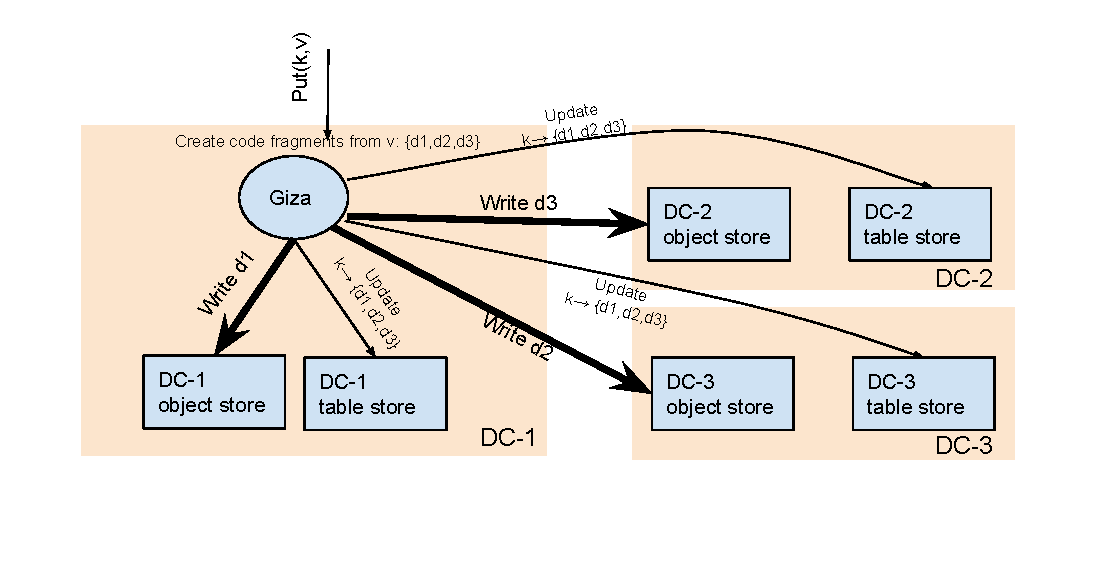
\includegraphics[width=0.5\textwidth]{fig/Giza}
\caption{Giza architecture\label{fig:arch}}
\end{figure}

\paragraph{Architecture}
{\name} is a global-scale cloud storage systems that span across many
datacenters in the world.  \name stores mutable, versioned objects.
~\Cref{fig:arch} shows the architecture of \name.  To support mutable coded
objects, \name separates the data path from meta-data path.  On the data-path,
object data is coded into several fragments, named by their content hashes, and
stored in the different DCs.   On the meta-data path, \name stores the set of
content hashes of coded fragments as the new version information for the object.

We take the approach to layer \name on top of existing cloud storage infrastructure. This 
provides two advantages.  First, doing so allows the rapid prototyping of \name by re-using 
mature, deployed systems.  Second, it simplifies the failure recovery and 
the deployment of \name, as \name servers are completely stateless and can be
readily integrated with the rest of the stateless cloud storage frontend.
Existing cloud storage systems have redundancy within a single data center, but
are not geo-replicated.  Thus, \name must explicitly provide cross data center
redundancy through coding and replication.  To write to an object, {\name}
stores coded fragments in cloud blob stores in different data centers, such as
Azure's blob store, or Amazon's S3.  Additionally, \name updates the object's
meta-data information (e.g.  versions, names of coded fragments for the new
content) in existing cloud tables and replicates them across several data
centers.  The number of coded fragments, and thus the set of data centers
storing object data, is configurable depending on the user desired tradeoff on
durability vs. cost.  The number of data centers to replicate the meta-data is
fixed at 3.

%blob service as building blocks, to store metadata and data respectively. This evolutional
%design allows {\name} to minimize footprint of new code. In fact, {\name} merely needs to replace the previous front-end
%module. With {\name} deployed, the user request comes in to the new frontend, where the new
%{\name} service will translate the user requests into a few metadata operations and data operations.
%
%In {\name}, both metadata and data are synchronously duplicated across different
%datacenters in order to tolerate datacenter failures. What is different between metadata
%and data is, metadata is fully replicated across a (usually smaller) set of datacenters using
%a tailored Fast-Paxos algorithm, persistent in the table service in each datacenter, thus
%tolerating a minority of failures; On the other hand, data in user request is encoded to
%a configurable number of fragments and shipped to a (usually larger) set of datacenters,
%persistent in the blob storage service. We refer the former as metadata path and the latter
%as data path.


\paragraph{Technical challenges}
In designing \name, we address three main technical challenges facing the basic approach.
\begin{enumerate}

\item {\it Building a strongly consistent, geo-replicated meta-data storage out of existing 
single-DC cloud tables.}  There are existing geo-replicated,
strongly-consistently storage systems (Cassandra, CockcoarchDB) that have been
built from the scratch.  However, we choose not to use them because we want to
keep \name servers stateless and keep all data and meta-data in existing
storage infrastructure that are operated by cloud providers. The common
technique to ensure strong consistency is to implement the Paxos protocol.  How
to implement Paxos using existing cloud storage APIs and achieve 
good performance in the cross-DC setting?

\item {\it Jointly optimizing the data and meta-data paths to achieve a single
cross-DC roundtrip for each operation.}

\item {\it Performing garbage collection efficiently and promptly.}

\end{enumerate}

%The separation of metadata path and datapath bring in the challenge that the consistency level
%could be violated with brutal yet flawed merge of the two. Our protocols described in later
%sections will guarantee the metadata path and data path together (especially when they are
%fully concurrent) will still provide a strong consistency insurance.
%


% A typical giza architecture for a data center includes the giza nodes, the Azure Blob Storage, and the Azure Table Storage. The giza nodes are the processing units of the Giza architecture and manages the data and the metadata. Furthermore the giza nodes participate in paxos rounds as coordinators. Figure 1 illustrates the architecture of Giza. Giza separates data from metadata and handles them on different paths. The data path is responsible for encoding the data and sending the data fragments across data centers. Each data fragment is stored in the corresponding DC’s Azure Blob Storage. The metadata path is responsible for storing the latest version of the data and the location of its data fragments. Giza uses a variant of the Paxos state machine replication (SMR) to maintain consistency of the metadata where each metadata server maintains a local copy of the replicated log. The replicated log is stored in the Azure Table Storage.

\subsection{Implementing Paxos using Cloud Storage APIs}

On the meta-data path, a \name node implements the Paxos protocol.

{\bf Meta-data storage layout.}
Before going into the protocols of {\name} operations, we first demonstrate our metadata
scheme. The metadata of an object is a row with a unfixed number of columns, as shown
in~\Cref{fig:xxxxx}. {\name} uses a version number to distinguish overwrites upon the same
object, so the metadata contains a column \texttt{highest\_committed\_version}, which is
a hint of which version is the latest modification, a.k.a. the decided version. It is named
as \texttt{highest\_committed\_version} rather than \texttt{highest\_version} to avoid the
ambiguity that the version may not be highest \emph{ongoing} version. Actually, the
\texttt{highest\_committed\_version} may not even be the real highest committed version at
the moment, but rather a hint that this version is possibly the highest committed version.

In addition to the \texttt{highest\_committed\_version}, the metadata needs to store the
location information of data fragment for each version. The location information contains
the coding configurations, which datacenters store the original/parity fragments, the keys
to retrieve those fragments in each blob service.

{\bf Meta-data Update.}

{\bf Meta-data Read.}

{\bf The FastPaxos optimization.}
The metadata row is replicated in a number of datacenters using a variant of Fast-Paxos
algorithm. Instead of storing the states of Fast-Paxos elsewhere, {\name} made a design
choice to use the metadata row itself as a durable space to hold the Fast-Paxos states.
The advantage of this choice is that {\name} can reuse the table service as the persistence
layer for the state machine replication, making {\name} nodes themselves stateless. As a
result, {\name} node has much less to worry about failure recovery. When a {\name} node
is (suspiciously) failing, a new {\name} node can be launched as an replacement without
doing extra work to nullify the previous node. The new node can directly access the table
service to work. 

%The metadata for each object includes the latest modification to that object using a versioning scheme. The highest version corresponds to the latest modification and the decided value for the version. In addition, the metadata also includes the location of the data fragments for the latest version. The metadata is replicated using a variant of the Paxos state machine replication. Instead of having a single log recording all the executions, each object has a corresponding paxos log. Giza uses the fault-tolerant Azure Table to store the metadata where each entry in the table corresponds to an object. Figure 2 illustrates the schema of the metadata table. 

\subsection{Joint optimization of Data and Meta-date Operations}

{\name} supports three operations: put, get and delete. All of them require a key as
an argument to identify an object. put takes object content as an extra argument, get
returns object content (null if non-exist) as result. A delete operation is processed
as a special write, putting a tombstone in the object's metadata. The actual recycling
of disk content happens at garbage collection, which will be described in ~\Cref{sec:xxxx}.

\subsubsection{Put}

When the {\name} node receives a put request, it encodes the data to $k$ original fragments
and $m$ parity fragments. $k$ and $m$ are configurable. Then the node computes a content
hash for each fragment, and use the hash value as key to write each fragment to a separate
datacenter.

\sm {
  Hi Daniel, can you give me a few details about the hashing? e.g. hashing method,
  hashing result size, collision rate, etc.)
}

Concurrently with the above data path, the giza node enters a metadata path to persist
the metadata into the table service in each datacenter. The metadata path begins with
choosing a proper version number to run the Fast-Paxos algorithm. The version number needs
to be the next version to the most recent committed version. It is safe to use an outdated
version (in which case the {\name} node will be noticed later and retry with a higher one),
but it is unsafe to choose a higher one. {\name} node finds the proper version in an
optimistic fashion. It first reading the highest\_committed\_version in the local table,
then use it plus one as the chosen version number.

With version number chosen, the {\name} node sends out a PreAccept request to the table
service in each datacenter. The request is a conditional update, if the metadata row
does not see any other update request on that version, it will acknowledge OK, otherwise
it will reply NACK. If the {\name} node receives a fast quorum of replies OK, it considers
the update on the metadata with that version successful. To accelerate later get operations,
the {\name} node sends out Commit requests to all datacenters, including those that
have not replied or replied NACK, in the background. The commit request is also a conditional
write; it updates the status of this version to committed, sets the highest committed
version to this version if not higher, and finalize the location information of data
fragments.

The above one-round trip metadata path is refer as fast path (The commit is in background,
so only PreAccept is counted as critical path). In the normal case without contention
the fast path should always succeed (We will discuss the counter case later). After the
fastpath is successful, the {\name} waits until the datapath finishes if it has not.
After both of metadata and datapath finishes, the {\name} node can acknowledge the client.
Assuming the across datacenter bandwidth is unbounded, the {\name} put operation commits
in one wide-area roundtrip.

In case of contention, the fast-path may not succeed. The contention may come from concurrent
{\name} put operations on the same object, or a failure recovering {\name} node trying to
re-commit the same or a different value to an ongoing version. {\name} will fall back to
classic Paxos to guarantee safety in case of contention.

If a {\name} node cannot collect a fast quorum of OK acknowledgement for the PreAccept requests,
or whenever a different {\name} node tries to do failure recover, it enters what is referred
as \emph{slow path}.To begin with, the {\name} node will pick a distinguished ballot number
that it thinks is large enough and send out a Prepare request with that ballot to all metadata
tables and wait for at least a majority of responses. The Prepare request is a mix of conditional
update and read operation. Each read request should return the entire metadata row at corresponding
datacenter. Upon a majority of replies, the {\name} needs to pick a value to try to commit.
The rules for picking the value is as follows. First it looks for the highest accepted ballot
in the replies. If there is one, the value from the reply is picked. If there is no accepted
value, but there is pre-accepted value, the {\name} node will pick the pre-accepted value
that appears more than others (if any) from the replies. If there is neither pre-accepted
nor accepted value. The {\name} node can pick any value it wants, e.g. the value it receives
from client or a \texttt{no-op} placeholder in failure recovery.

After the {\name} node picks a value, it sends out Accept request to all metadata tables.
An Accept request is a conditional update, if the max\_ballot\_seen is smaller, it updates
the max\_ballot\_seen, writes the picked value to the version. After {\name} node collects
a majority of successful acknowledgements for the Accept requests, it succeeds in writing
the metadata and may return to the client after the datapath is also done. A commit phase
similar to above is launched in background.

\subsubsection{Get}
When {\name} receives a get request, it decompose the request to metadata path and datapath
as well, similar to the put operation. A regular (but slower) way to do this is serialize
metadata path and datapath. Before retrieving the data fragments, the {\name} needs to
get the metadata for the most recently committed version. While this is effective,
it incurs at least one across datacenter roundtrip before it can starts to retrieve the
actual data, which is also located in a different datacenter, which could hurt latency
performance.

Instead, {\name} chooses an optimistic style to parallelize the metadata and data path.
On get request, a {\name} first read from local datacenter table service, requesting
the metadata row. From the row it reads the highest\_committed\_version and its data
fragments location information. Then it starts to read the data fragments from different
datacenter. After enough pieces received, the {\name} node can reconstruct the original
data and have it standby to reply to the client.

Separately, the {\name} launches a metadata path to validate the version above is actually
the correct version to read. It reads the metadata row from all datacenter and expect
at least a majority of replies. If among the replies it has not observed any higher ongoing
version that has any accepted value, the {\name} node can safely return the standby
data because it is guaranteed to be the latest committed value.

If unfortunately the {\name} node observes a higher version with accepted value in the
replies, it needs to try a slowpath in the put operation above to confirm on that version
because it could possibly be considered committed once before. After it succeed in
the slow path, the {\name} node needs to re-launch the datapath to retrive the data
fragments of the newer version and abandon the old ones. This serialized metadata and
datapath case typically happens when there is concurrent read and write on the same
object, which is rare in our workload.

\sm{ Hi Daniel, just want to confirm, is this what you do now? Only one accepted
  in higher version will invalidate the optimistic read}

There is a rare case that a {\name} node could read a committed version from metadata,
however the data fragments has not been written to the blob storage. This is due to
the metadata path in the put operations could finish before the data path. In this case,
the {\name} node in the get operation needs to recursively fall back to the previous
version. That said, the highest\_committed\_version could either higher or lower than the actually
``committed'' version.
  
\subsection{Conditional Write}
The protocols above strongly depend on the conditional write feature provided by the
table service. Some of the cloud providers already support this feature, such as Amazon.
Other coud providers usually provide alternative functions. For example, as used in our
experiments, Windows Azasure provides a function called ETag. An ETag works similar to
a lease. It is generated at the table service side and returned to a table service client
on a read request. The client could give the tag as an argument in later write operations,
and the writes will only succeed if the row was not accessed by another client.

For Azure-like system, {\name} implements conditional write based the ETag feature.
However, an across datacenter conditional operation based ETag may still incur multiple
roundtrips. To optimize the latency, we introduce the \emph{delegation} mechanism
into {\name}. To issue an across site conditional operation, a {\name} node delegates the
request to another {\name} node in the remote datacenter, the remote {\name} works as
a proxy to finish the operation and returns the result. This optimization will largely
reduce the latency result. Because all the requests can be safely abandoned and retried,
the {\name} nodes are still stateless with delegation.

\subsection{Garbage Collection}
Because {\name} keeps writing new version metadata to table service and data fragments
to blob storage service, it needs to garbage collect on outdated versions to recycle
storage space. Moreover, the garbage collection also needs to free the space marked as
tombstone by the delete operation.

Recycling the old versions data includes deleting the data and parity fragments and
truncating the columns for the old versions in the metadata row. Garbage collection
for an object follows three steps: 1) read the metadata row and get the columns to
delete based on the \texttt{hightest\_committed\_version}. 2) send delete requests to
blob storage service to delete the data. 3) remove the columns for the old versions
in the table service. The second step has to happen before the third in case that the
garbage collection process is interrupted and the data fragments may become ``orphans''
without proper metadata to point to them in the table service.

After a delete operation, {\name} sees the row marked as tombstone by a special column.
Now it needs to remove the entire row, which requires extra care. Otherwise if removed
brutally, another put operation on the same key may bring the system into an abnormal
state. The new put operation will start with the initial version again, which could
violate some of the metadata (with a higher version before the deletion) if the removing is still in
process. Therefore, {\name} chooses to use two-phase commit when to remove the metadata
row. In the first phase, it marks the rows in all datacenters as ``prepared\_to\_delete''.
After this any other get or put operations are temporarily disabled on this row. Then
in the second phase, all the rows are actually removed from the table service. The
disadvantage for this approach is that it requires all datacenters online. Any crashed
datacenter or network partition may pause the process and makes the row unavailable
(but can still continue or recovered after the failure is eliminated). 


\section{Reconfiguration}
\subsection{Datacenter Failures}

\subsection{Viewchange}

\subsection{Migration}

% \subsection{Giza Workflow}
% Because of the high WAN RTT, Giza’s primary goal is to minimize the number of round trips in its put and get critical paths while maintaining strong consistency semantics. By approaching this problem with multiple iterations, we were able to reduce the original 3  WAN RTT to 1 WAN RTT in most cases, dramatically reducing the put and get latency.

% \subsubsection{3 RTT Put and Get}
% Figure 3 illustrates the workflow of a typical Put operation. When a client issues a Put command, Giza first queries its local metadata to identify a most likely latest version of the object. It then starts a paxos round for the version. A paxos round is broken down into two phases: the prepare phase and the accept phase. Giza runs the data path first, where the object is erasure encoded and the data fragments are sent to the corresponding data centers. (Here, we have to write this information down in case of giza node failure right). When the data path returns successfully, Giza proceeds to run the metadata phase which incurs two round trips.
% \par 
% During the Get path, Giza runs the metadata phase first to get the location of the data fragments. To ensure a consistent latest version of the data, Giza runs a paxos round for get on the object’s entry log. When this succeeds, Giza runs the datapath and receives enough data fragments to reconstruct the original data before returning to the client. Both the Put and Get incurs two rounds in the metadata path and 1 round in the data path.

% \subsubsection{2 RTT Put and Get}
% We quickly realized that the separation of metadata path and data path allows for some parallelism. In particular, during the Put path, Giza can run the prepare phase of the metadata path in parallel with the data path. When prepare phase and the data path succeed, Giza runs the second phase of the paxos round. Once this round completes, Giza can return acknowledgement to the client. This brings the round trips down to 2 round trips in the optimal case.
% \par
% Furthermore, during Get, Giza can run the additional paxos round for the get operation in parallel with the data path get. This can be done by first optimistically assuming that the current highest entry of the object in its local entry log is in fact the highest version. Once this information is obtained, Giza can then proceed to get the data fragments while simultaneously validating the consistency of the latest version on the metadata path. If the assumption is correct, the Get incurs 2 round trips.

% \subsubsection{1 RTT Put and Get}
% We used the classical Paxos protocol for achieving consistency on our metadata path. [Introduce Fast Paxos and why this works in this case, should do this after reading in depth about Fast Paxos]. This reduces Giza’s put path to 1 round trip.
% \par
% In the Get Path, we realized that we can forego running the paxos round in some scenarios by including a learning phase on the non-critical path of Put. After acknowledging to the client’s put request, the coordinator giza node will send the accepted version and the version number as a committed entry for the object to the other participating giza nodes. This entry is used to serve as the highest committed version and will only override existing entry if the version is higher. During a client’s Get request, Giza first obtains the object’s row entry from the majority of the participating giza nodes. If the latest entry in the paxos log are consistent or not higher than the highest committed entry, then Giza can safely return the results obtained from the data path. However, in the case where the latest entry in the paxos log is higher than the highest committed entry (This can happen if the giza nodes are simultaneously performing a paxos round for a newer version of the object or the learning phase has not reached the giza nodes), then Giza can still get the highest version but doing two things. First it can fallback to the previous approach of running a paxos round for the get operation. Alternatively, it can wait to obtain the object’s row from all the participating giza nodes (instead of the previous majority). In our scheme, we execute both options concurrently and return once the faster of the two approaches completes.

% \subsection{Giza Recovery}
% Describe the mechanism of recovery when a data path node fails but a metadata path node doesn’t (6-1 scheme still only utilizes 3 giza nodes for metadata).
% \par
% Describe the mechanism when a DC containing both data path and metadata path node fails (membership change).

%%% Local Variables:
%%% mode: latex
%%% TeX-master: "main"
%%% End:

